\documentclass[]{article}

\usepackage[autostyle]{csquotes}  
\usepackage{graphicx}
\graphicspath{{images/}}


\newcommand{\goto}{\texttt{->} \textbf{goto}  }

\author{Marco Favorito 1609890}
\title{%
Denial-of-Service on Tendermint \\ 
\large Seminars in Advanced Topics in Computer Science Engineering 2016/2017}

\begin{document}

\maketitle
\tableofcontents

\section*{Introduction}
In this report I describe an experimental Denial-of-Service attack against the Tendermint protocol, using Ethermint as ABCI application.

In Section \ref{toverview} I summarize the main features of Tendermint and how it works;

In Section \ref{tcap} I analyze the Tendermint protocol wrt CAP properties;

In Section \ref{tevil} I describe the type of DoS attack I designed and how the byzantine node for the DoS attack has been implemented;

In Section \ref{bench} I show how the byzantine node affects the Tendermint network performances.

\section{Tendermint overview}
\label{toverview}

In this section we explore Tendermint in its components and its consensus algorithm.
\subsection{What is Tendermint}

Tendermint \cite{tpaper, tthesis, tdocs} is a software for Byzantine fault-tolerant (BFT) state machines replication, powered by blockchain-based consensus. It is secure, since allow to 1/3 of nodes to fail, and consistent, since every correct node agree on the same state of the application.

The two main component of Tendermint are:
\begin{itemize}
	\item Tendermint Core: consensus engine
	\item Application BlockChain Interface (ABCI): enables the transactions to be processed in any programming language

\end{itemize}

\subsection{How ABCI works: message types}
Tendermint Core interacts with the application via a socket protocol that satisfies ABCI.
The message types exchanged by nodes are many. The more important are:

\begin{itemize}
	\item \textbf{DeliverTx}: with which every transaction is delivered in the blockchain. Application needs to validate each transaction received with the DeliverTx message against the current state;
	\item \textbf{CheckTx}: used for validate transactions, before entering into the mempool;
	\item \textbf{Commit}: used to compute a cryptographic commitment to the current application state, to be placed into the next block header.
\end{itemize}

Tendermint Core creates three ABCI connections to the application:
\begin{itemize}
	\item for validating transactions to put into the mempool;
	\item for run block proposals for the consensus engine;
	\item for querying the app state.
\end{itemize}

\subsection{How Tendermint Core works: the consensus algorithm}
Tendermint Core manages the Proof-of-Stake consensus algorithm to commit the incoming transactions in the blockchain. 

In this section I state the working assumptions and the consensus phases of the algorithm.

\subsubsection{Working assumptions}

The working assumptions, in order to allow the algorithm to work, are \cite[Section 6.1: On Byzantine Consensus]{tpaper}:
\begin{enumerate}
	\item \textbf{Assumption 1}: The network is partially synchronous;
	\item \textbf{Assumption 2}: All non-byzantine nodes have access to an internal clock that can stay sufficiently accurate for a short duration of time until consensus on the next block is achieved; The clocks do not need to agree on a global time and may drift at some bounded rate relative to global time.
	\item \textbf{Assumption 3}: At least $2/3$ of the voting power is honest.
\end{enumerate}

\paragraph{Motivations of the working assumptions}
\begin{enumerate}
	\item When the Assumption 1 fails, no consensus is possible. This result is known as the FLP impossibility result \cite{flp}. 
	
	\item The Assumption 2 is needed in order to ensure that eventually the consensus procedure at a certain height is completed. Key statements to see this are:
	
	\begin{itemize}
		\item Each round is longer than the previous round by a small fixed increment of time. This allows the network to eventually achieve consensus in a partially synchronous network \cite[Section 6.2]{tpaper};
		\item The asynchronous and local nature of CommitTime allows the network to maintain consensus despite drifting clocks, as long as the clocks remain accurate enough during the consensus process of a given height \cite[Section 6.2]{tpaper};
	\end{itemize} 
	
	
	In other words, there is no need of global time synchronization, but the drift has to be bounded to allow the timeout mechanism to work. Eventually, the timeouts become big enough to allow the messages to be delivered in time for an enough number of nodes. Clocks do not need to be synced across validators, as they are reset each time a validator observes votes from two-thirds or more others.
	
	
	\item Assumption 3 ensures \textit{safety} and \textit{liveness}. We will deepen the analysis in Section \ref{tcap}.
\end{enumerate}

\subsubsection{Consensus phases}
There are 3 phases (\textbf{Propose}, \textbf{Prevote}, \textbf{Precommit}) plus 2 special phases, \textbf{Commit} and \textbf{NewHeight}.\\
A \textbf{Round} is defined as:

\begin{verbatim}
Propose -> Prevote -> Precommit
\end{verbatim}

In the optimal scenario, the order of steps is:
\begin{verbatim}
NewHeight -> Propose -> Prevote -> Precommit+ -> Commit -> NewHeight ->...
\end{verbatim}
Why things might go wrong? Some examples:

\begin{itemize}
\item The designated proposer was not online.
\item The block proposed by the designated proposer was not valid.
\item The block proposed by the designated proposer did not propagate in time.
\item The block proposed was valid, but +2/3 of prevotes for the proposed block were not received in time for enough validator nodes by the time they reached the Precommit step. Even though +2/3 of prevotes are necessary to progress to the next step, at least one validator may have voted <nil> or maliciously voted for something else.
\item The block proposed was valid, and +2/3 of prevotes were received for enough nodes, but +2/3 of precommits for the proposed block were not received for enough validator nodes.
\end{itemize}
The common exit conditions for the algorithm are:
\begin{itemize}
\item After +2/3 precommits for a particular block. \goto Commit(H)
\item After any +2/3 prevotes received at (H,R+x). \goto Prevote(H,R+x)
\item After any +2/3 precommits received at (H,R+x). \goto  
Precommit(H,R+x)
\end{itemize}
Now I briefly describe every phase of the state machine behind the Tendermint protocol. The specification is mainly taken from \cite{tdocs}.

\paragraph{Propose (height H, round R)} Upon entering Propose, the designated proposer proposes a block at height H and round R.

The proposer is chosen by a deterministic and non-choking round robin selection algorithm that selects proposers in proportion to their voting power. (see implementation). A \textbf{Proposal} is constituted by:
\begin{itemize}
\item a block
\item an optional latest PoLC-Round $<$ R (proof-of-lock-change) which is included iff the proposer knows of one. This hints the network to allow nodes to unlock (when safe) to ensure the liveness property
\end{itemize}
A proposal is signed and published by the designated proposer at each round.
\\
Exit conditions:
\begin{itemize}
	\item After timeoutProposeR after entering Propose. \goto  Prevote(H,R)
	\item After timeoutProposeR after entering Propose. \goto  Prevote(H,R)
	\item After receiving proposal block and all prevotes at PoLC-Round. \goto Prevote(H,R)
	\item After common exit conditions.
\end{itemize}


\paragraph{Prevote Step (height H, round R)} Upon entering Prevote, each validator broadcasts its prevote vote.

First, if the validator is locked on a block since LastLockRound but now has a PoLC for something else at round PoLC-Round where $LastLockRound < PoLC Round < R$, then it unlocks.\\
If the validator is still locked on a block, it prevotes that.\\
Else, if the proposed block from Propose(H,R) is good, it prevotes that.\\
Else, if the proposal is invalid or wasn’t received on time, it prevotes \textit{nil}.\\

The Prevote step ends:
\begin{itemize}
\item After +2/3 prevotes for a particular block or . \goto Precommit(H,R)
\item After timeoutPrevote after receiving any +2/3 prevotes. \goto Precommit(H,R)
\item After common exit conditions
\end{itemize}

\paragraph{Precommit Step (height H, round R)} Upon entering Precommit, each validator broadcasts its precommit vote.\\
If the validator has a PoLC at (H,R) for a particular block B, it (re)locks (or changes lock to) and precommits B and sets LastLockRound = R.\\
Else, if the validator has a PoLC at (H,R) for \textit{nil}, it unlocks and precommits \textit{nil}.\\
Else, it keeps the lock unchanged and precommits \textit{nil}.\\
A precommit for \textit{nil} means ``I didn’t see a PoLC for this round, but I did get +2/3 prevotes and waited a bit".

The Precommit step ends:
\begin{itemize}
\item After +2/3 precommits for \textit{nil}. \goto Propose(H,R+1)
\item After timeoutPrecommit after receiving any +2/3 precommits. \goto Propose(H,R+1)
\item After common exit conditions
\end{itemize}

\paragraph{Commit Step (height H)} Set $CommitTime = now()$ and wait until block is received. \goto NewHeight(H+1)\\


\paragraph{NewHeight Step (height H)}
Move $Precommits$ to $LastCommit$ and increment $height$,
set $StartTime = CommitTime+timeoutCommit$ and wait until $StartTime$ to receive straggler commits. \goto Propose(H,0)
\\
\\
In Figure \ref{messages} is depicted the message passing schema:
\begin{figure}[h]
\centering
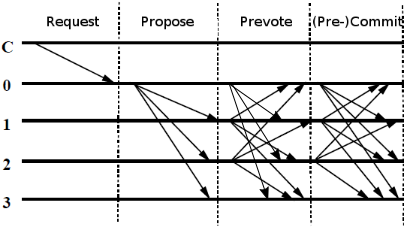
\includegraphics[width=0.8\textwidth]{tendermint-messages}
\caption{\label{messages} Message passing schema for the Tendermint consensus algorithm.}
\end{figure}
\\

\subsection{What is Ethermint}
Ethermint\footnote{\texttt{https://github.com/tendermint/ethermint}} it is an app that:
\begin{itemize}
	\item It implements the logic of Ethereum
	\item It is ABCI-compliant
\end{itemize}
All consensus stuff is managed by Tendermint Core.

\section{Tendermint and the CAP Theorem}
\label{tcap}
In this section we follow the same approach used in \cite{poa-vs-pbft}.

The CAP properties (namely, \textit{Consistency}, \textit{Availability} and \textit{Partition Tolerance}) in blockchain applications are interpreted as the following:
\begin{itemize}
\item Consistency: A blockchain achieves consistency when forks are avoided.
\item Availability:A blockchain is available if transactions submitted by clients are served and eventually committed, i.e. permanently added to the chain.
\item Partition Tolerance: When a network partition occurs, Tendermint validators are divided into disjoint groups in such a way that nodes in different groups cannot communicate each other.
\end{itemize}
Since a blockchain must tolerate partitions, hence CA option is not considered, we analyse the algorithms with respect to CP and AP options.

\subsection{Analyzing Consistency}
As stated in \cite{tpaper}:
\blockquote{
A block is considered committed when a 2/3 majority of validators sign commit votes for that block. A fork occurs when two blocks at the same height are each signed by a 2/3 majority of validators. By simple arithmetic, a fork can only happen when at least a 1/3 majority of validators signs duplicitously.}
Hence, as long as there exists a majority of honest validators, in terms of their voting power, no forks can happen (see Assumption 3 in Section \ref{toverview})

More formally, Tendermint ensures Safety and Liveness \cite[Section 6.3 and 6.4]{tpaper} as long as $N \ge 3f + 1$\footnote{NOTICE: numbers in the inequality must be intended in terms of voting power and not in terms of number of nodes.}.
The property are stated as the following:
\begin{itemize}
\item \textbf{Safety property}: If there are less than 1/3 in Byzantine voting power and at least one good validator decides on a block $B$, then no good validator will decide on any block other than $B$. 

\item \textbf{Liveness Property}: If there are less than 1/3 in Byzantine voting power then this protocol does not deadlock.
\end{itemize}
This property underlines the similarities with PBFT, more precisely on the optimal resiliency (see Section 3 "Service Properties" in \cite{pbft}).

The differences with PBFT are \cite[Section 10.2.4]{tthesis}):
\begin{itemize}
\item No fixed primary node: the proposer changes every blocks;
\item The use of blocks allows Tendermint to include the set of pre-commit messages from one block in the next block, removing the need for an explicit commit message.
\item Accountability guarantees when forks or some bad behaviors happen \cite[Section 3.5]{tthesis}.
\end{itemize}

\subsection{Analyzing Availability}
As stated in \cite[Section 3.2: Consensus]{tthesis}:
\blockquote{
	After the proposal, rounds proceed in a fully asynchronous manner - a validator makes progress only after hearing from at least two-thirds of the other validators. This relieves any sort of dependence on synchronized clocks or bounded network delays, but implies that the network will halt if one-third or more of the validators become unresponsive.}

In other words, if Assumption 1 does not hold (i.e. delays are unbounded), the algorithm simply halts.
\subsection{Conclusions}
When the assumption on the network fails, consistency is preserved while availability is given up. Hence, Tendermint can be classified as CP system, according to the CAP theorem.

\section{DoS: Tendermint Evil}
\label{tevil}
In this section we describe the types of Denial-of-Service attacks developed for the project, showing how I've modified the source code of Tendermint\footnote{\texttt{https://github.com/tendermint/tendermint}} to accomplish them.

For each type of attack there is a modified version of Tendermint named \textit{Tendermint Evil - $<$version-name$>$}. In order to implement them I forked\footnote{\texttt{https://github.com/MarcoFavorito/tendermint}} the original Tendermint repository.

\subsection{Tendermint Evil `Silent'}
This attack\footnote{\texttt{https://github.com/MarcoFavorito/tendermint/releases/tag/v0.12.1.1}} is very straightforward: it simply make the byzantine node to do not send any message in the network to the other peers.

The modified source code file is \texttt{p2p/connection.go}, in which the core functions \texttt{Send} and \texttt{TrySend} have been 'neutralized': I've commented out the lines of code which actually send bytes to the other peers.

More specifically, the main changes is:
\begin{itemize}
\item In \texttt{Send()}:
\begin{verbatim}
-    success := channel.sendBytes(wire.BinaryBytes(msg))
+    //success := channel.sendBytes(wire.BinaryBytes(msg))
+    success:=true
\end{verbatim}
\item In \texttt{TrySend()}
\begin{verbatim}
-    ok = channel.trySendBytes(wire.BinaryBytes(msg))
+    //ok = channel.trySendBytes(wire.BinaryBytes(msg))
\end{verbatim}
\end{itemize}

In simple words, we deceive the program by simulating a successful send, so the state machine execution is not affected.

This version has not been very useful for the DoS. The problem that makes the attack not effective is that the byzantine does not respond to heartbeat messages. Hence, the connections between the other peers and the byzantine node are quickly dropped because the correct nodes wisely ignore another node if it becomes unresponsive.

\subsection{Tendermint Evil `Shy'}
\label{shy}
This version\footnote{\texttt{https://github.com/MarcoFavorito/tendermint/releases/tag/v0.12.1.2}} is a bit smarter than the previous one: it sends heartbeat messages but do not sends any block or proposals (when it is designed as proposer for the current round) and votes.

The main changes are in \texttt{consensus/state.go}:
\begin{itemize}
	\item In \texttt{defaultDecideProposal()}\footnote{Some parts have been omitted in order to help readability. Please refer to }:
	\begin{verbatim}
	-    cs.sendInternalMessage(msgInfo{&ProposalMessage{proposal}, ""})
	-    for i := 0; i < blockParts.Total(); i++ {
	-    	part := blockParts.GetPart(i)
	-    	cs.sendInternalMessage(...)
	-    }
	-    cs.Logger.Info("Signed proposal" ...)
	-    cs.Logger.Debug(cmn.Fmt("Signed proposal block: %v", block))
	+    //cs.sendInternalMessage(msgInfo{&ProposalMessage{proposal}, ""})
	+    //for i := 0; i < blockParts.Total(); i++ {
	+    //	part := blockParts.GetPart(i)
	+    //	cs.sendInternalMessage(...)
	+    //}
	+    //cs.Logger.Info("Signed proposal" ...)
	+    //cs.Logger.Debug(cmn.Fmt("Signed proposal block: %v", block))
	+
	+    cs.Logger.Info("EVIL! Do not send proposal.")
	\end{verbatim}
	\item In \texttt{signAddVote()}
	\begin{verbatim}
	-    cs.sendInternalMessage(msgInfo{&VoteMessage{vote}, ""})
	-    cs.Logger.Info("Signed and pushed vote" ...)
	+    //cs.sendInternalMessage(msgInfo{&VoteMessage{vote}, ""})
	+    //cs.Logger.Info("Signed and pushed vote" ...)
	+    cs.Logger.Info("EVIL! Do not send vote")	
	\end{verbatim}
\end{itemize}
The main purposes of this version are:
\begin{itemize}
\item Weaken the network: another node failure blocks the consensus algorithm (no enough voting power to commit blocks);
\item Delay the commit phase: when at some height the byzantine node becomes the proposer, the algorithm is delayed about the $timeoutProposeR$ since no proposal is made. After the timeout, the round-robin algorithm select another node, and the algorithm moves to a new round (but same height).
\end{itemize}

\subsection{Tendermint Evil `NoProposals'}
This attack\footnote{\texttt{https://github.com/MarcoFavorito/tendermint/releases/tag/v0.12.1.1}} is the same of Tendermint Evil `Shy', but sends votes and participate to the other phases of the consensus algorithm

The main purposes of this version is that, differently from the previous one, in case the byzantine nodes are more than the tolerable the algorithm still goes forward, but delayed more often.

\section{Experiments}
\label{bench}
In this section I briefly describe the experiments and show some results about the networks performances. The load test has been performed by Tsung\footnote{\texttt{http://tsung.erlang-projects.org/}}. The entry point for the Tendermint network setup is \texttt{ethermint-dos.py}\footnote{\texttt{https://github.com/MarcoFavorito/ethermint-dos/blob/master/ethermint-dos.py}}, that you will find at the root of the repository for this project\footnote{\texttt{https://github.com/MarcoFavorito/ethermint-dos}}. \\

We made 3 experiments:
\begin{enumerate}
	\item \textbf{No byzantine nodes}: a Ethermint/Tendermint network where every node is correct. More precisely, 4 correct nodes. We will refer to it later with the name \texttt{Normal}. The command executed is:
	\begin{verbatim}
	python3 ethermint-dos.py 4 0
	\end{verbatim}
	\item \textbf{Number of byzantine nodes $f < N/3$}: where the number of byzantine nodes is still tolerable. More precisely, 3 correct nodes and 1 byzantine node. We will refer to it later with the name \texttt{Evil\_1}. The command executed is:
	\begin{verbatim}
	python3 ethermint-dos.py 4 1
	\end{verbatim}
	\item \textbf{Number of byzantine nodes $f \ge N/3$}: where the number of byzantine nodes is greater than the tolerable (indeed the algorithm stop working). More precisely, 2 correct nodes and 2 byzantine nodes. We will refer to it later with the name \texttt{Evil\_2}. The command executed is:
		\begin{verbatim}
		python3 ethermint-dos.py 4 2
		\end{verbatim}
\end{enumerate}

\subsection{Setup}
The test for every experiment consists of the following steps:
\begin{enumerate}
	\item Set up the network (using \texttt{ethermint-dos});
	\item Start a Tsung load test session of 2 minutes and 5 users per second, where the sequence of requests (``Transaction" in Tsung jargon) is composed as the following:
	\begin{enumerate}
		\item send one transaction;
		\item do polling until the transaction is validated, but after 20 seconds exit the loop.
	\end{enumerate}
	The requests are directed to the Ethermint app, to only one node.
	\item Collect the results.
\end{enumerate}

\subsection{Results}

In Table \ref{bench-main} is shown the output of one of the session tests,  concerning the statistics of the requested transactions. 

\begin{table}[!htb]
\centering
\begin{tabular}{| l | l | l | l | l | l | l |}
	 \hline
	Name  & highest 10sec mean  & lowest 10sec mean & Highest Rate & Mean Rate & Mean  & Count \\
	 \hline
	 normal\_tx  & 6.15 sec & 4.10 sec & 5.9 / sec & 4.46 / sec & 4.81 sec & 552 \\	
	 \hline
	 evil\_1\_tx  & 7.65 sec & 3.97 sec & 7.4 / sec & 4.62 / sec & 5.60 sec & 600  \\
	 \hline
	 evil\_2\_tx  & 30.06 sec & 30.06 sec & 5.7 / sec & 4.06 / sec & 30.06 sec & 568  \\
	 \hline

\end{tabular}
\caption{\label{bench-main} Transactions statistics taken from the output of Tsung load tests.}
\end{table}
From Table \ref{bench-main} you can notice that:
\begin{itemize}
	\item the \textbf{highest mean} and \textbf{lowest mean}\footnote{i.e. respectively the highest and lowest mean duration of transactions sampled in windows of 10 seconds} range in the \texttt{Normal} case is narrower than the one in the \texttt{Evil\_1} case. This means that in the former case the system is more stable and predictable in terms of performances than the latter one.
	
	In the \texttt{Evil\_1} experiment there is no range: all the users wait the validation of the transaction for 20 seconds (which will never arrive since the algorithm does not proceed in validating blocks) and then exit with failure.
	\item the \textbf{highest rate} of transactions is higher in the \texttt{Evil\_1} case rather than the \texttt{Normal} case; This is due to the fact that the network is slower when the byzantine node is chosen as validator. Hence the pending transactions grow in number and are inserted in a block all together at one time. This eventually allow to reach higher transaction rate than the \texttt{Normal} network, since this one distributes pending transaction on more blocks at regular time intervals.
	
	In \texttt{Evil\_2} this parameter has no meaning, since no transaction is validated.
	
	\item the \textbf{mean} time of a transaction is slightly higher in the \texttt{Evil\_1} case than in the \texttt{Normal} case; this is an expected result, since the network with one byzantine node should be less responsive than the normal one.
	The value for the \texttt{Evil\_2} experiment is due to the fact that all the transactions end after a polling loop of 30 seconds.
\end{itemize}


In the graph shown in Figure \ref{simultaneous_users} we can see the number of simultaneous users connected to the server. The higher the number, the lower the responsiveness of the system to validate transactions. The reader can notice that the line of the \texttt{Evil\_1} setup is on average higher than the one of the \texttt{Normal} case.
\begin{figure}[h]
	\centering
	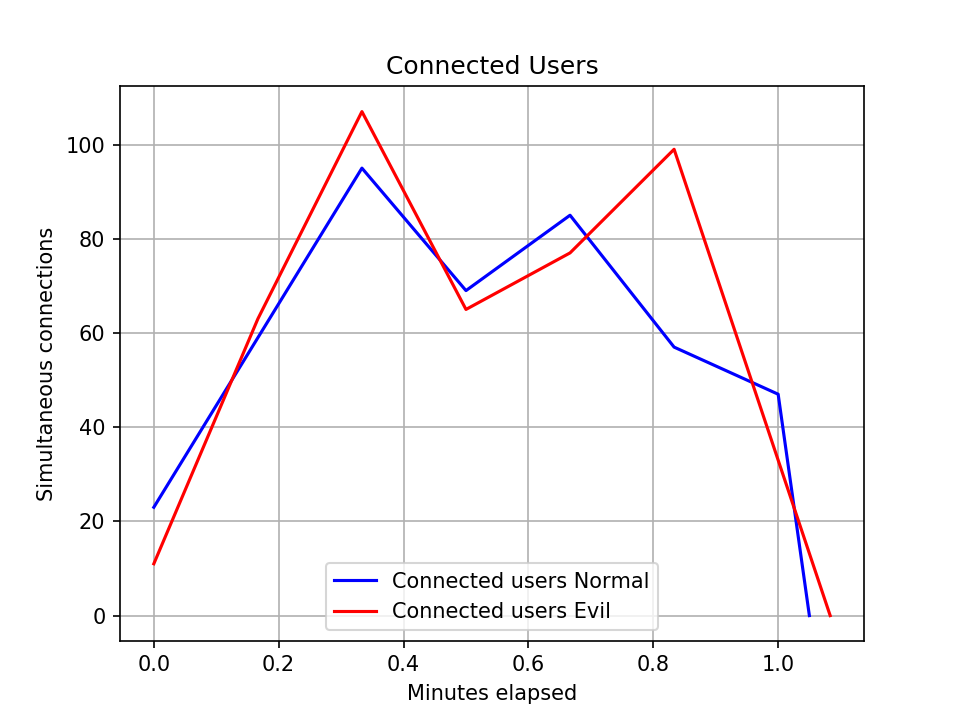
\includegraphics[width=0.8\textwidth]{simultaneous_users}
	\caption{\label{simultaneous_users} Simultaneous connected users}
\end{figure}

In Figure \ref{tm_normal}, \ref{tm_evil-1} and \ref{tm_evil-2} you can see, respectively, the Transaction duration over time for experiment \texttt{Normal}, \texttt{Evil\_1} and \texttt{Evil\_2}. In the first case, the duration of Transactions (i.e. the time to wait for validate a transaction) is more stable than the second case.
\begin{figure}[h]
	\centering
	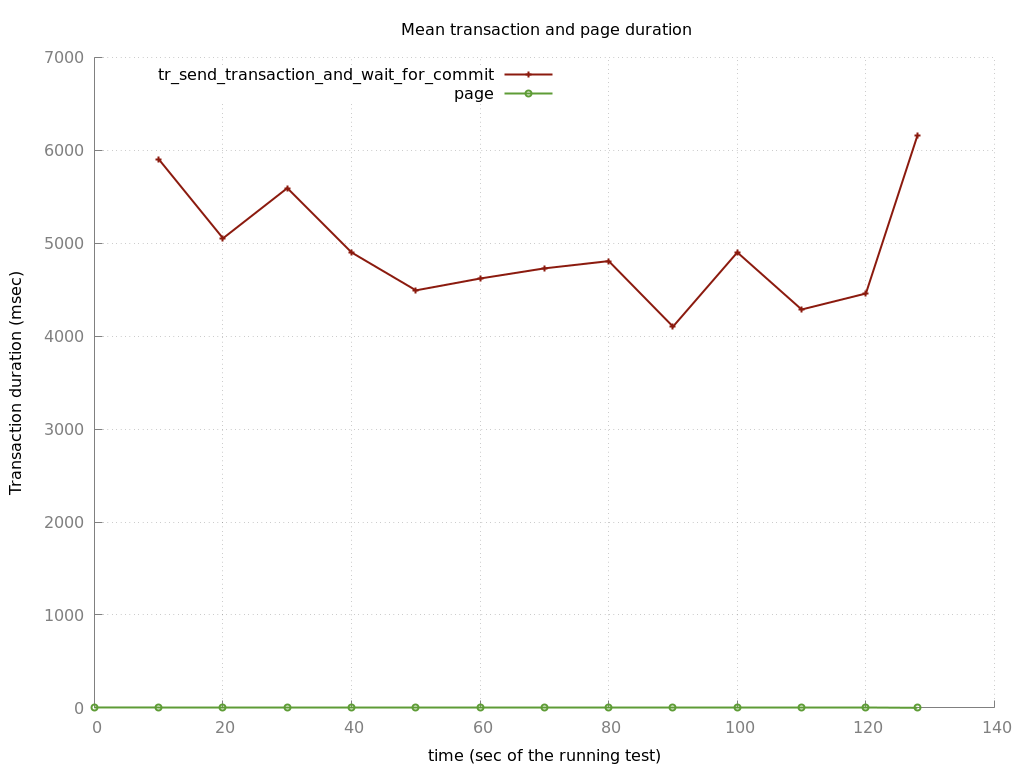
\includegraphics[width=0.8\textwidth]{images/graphes-Transactions-mean-normal.png}
	\caption{\label{tm_normal} Transaction duration over time for experiment \texttt{Normal}}
\end{figure}
\begin{figure}[h]
	\centering
	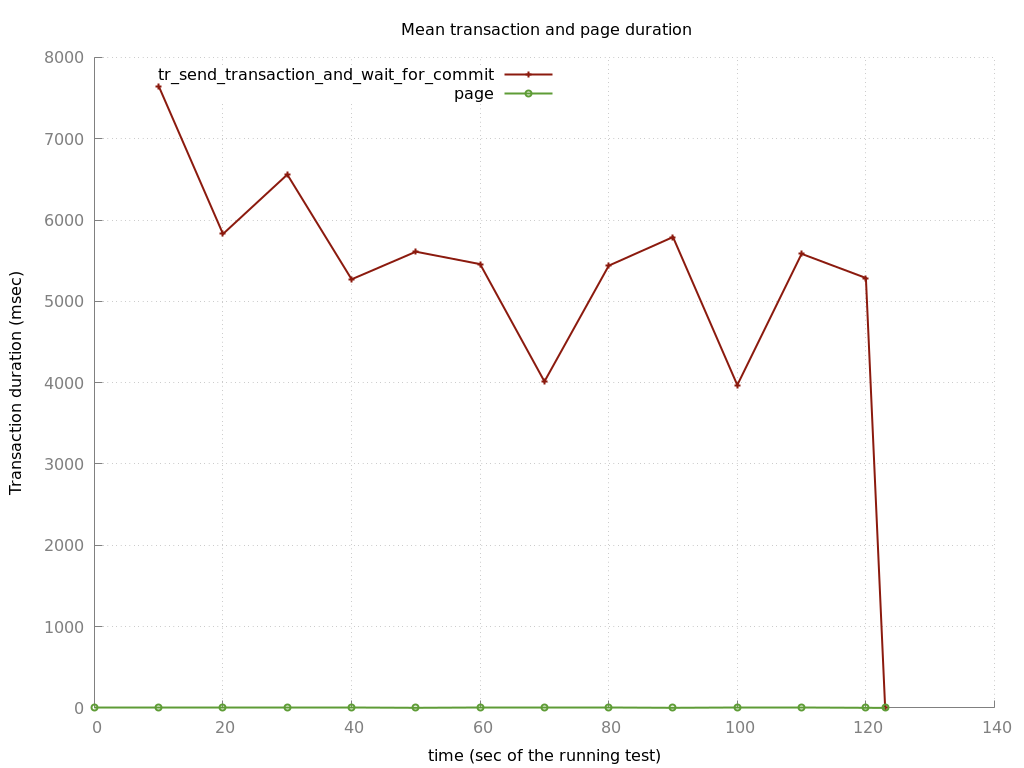
\includegraphics[width=0.8\textwidth]{images/graphes-Transactions-mean-evil_1.png}
	\caption{\label{tm_evil-1} Transaction duration over time for experiment \texttt{Evil\_1}}
\end{figure}
\begin{figure}[h]
	\centering
	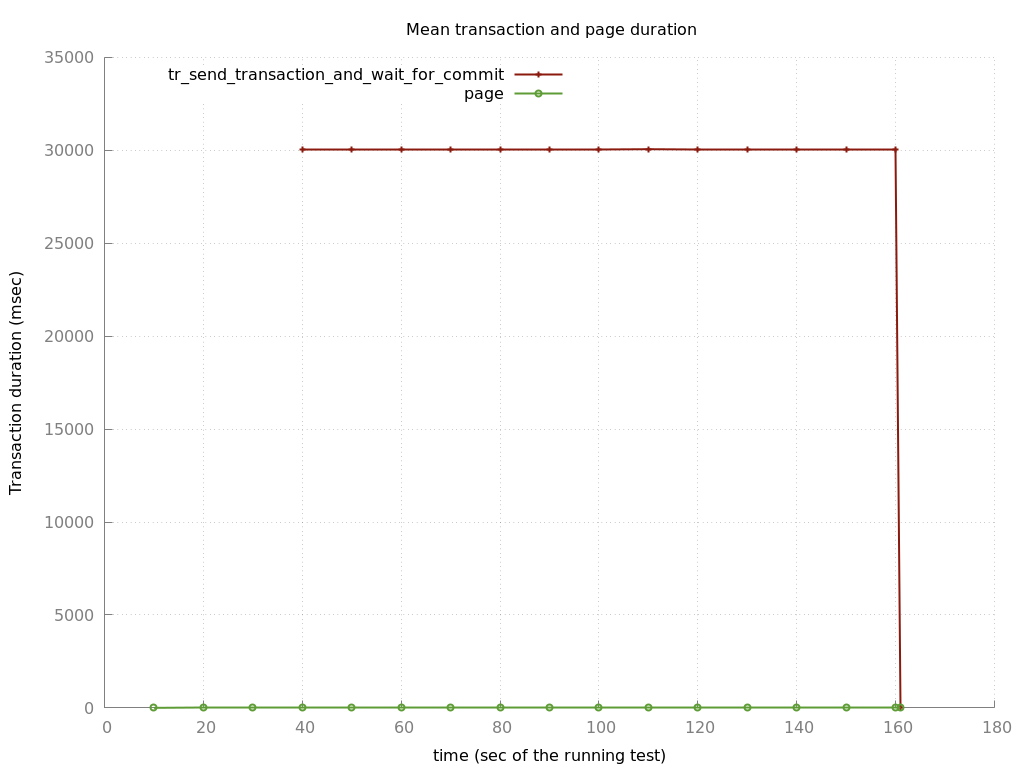
\includegraphics[width=0.8\textwidth]{images/graphes-Transactions-mean-evil_2.png}
	\caption{\label{tm_evil-2} Transaction duration over time for experiment \texttt{Evil\_2}}
\end{figure}


\section{Conclusions}
In this project I tried to perform a simple DoS attack against the Tendermint protocol. In Section \ref{toverview} I briefly describe the main Tendermint features, while in Section \ref{tcap} I analyzed the Tendermint algorithm froma theoretical point of view, using the CAP Theorem. In the experiment, the byzantine node does not send proposals and votes. As explained in Section \ref{shy}, the purpose is to delay the consensus algorithm. In Section \ref{bench} I showed quantitatively how this type of DoS attack affects the Tendermint/Ethermint network, leveraging Tsung functionalities.
In short, The performances of the network with one byzantine are slightly worsen, in particular about what concern the stability and predictability of the system.
\begin{thebibliography}{9}
\bibitem{tpaper}
	Tendermint: Consensus without Mining
\bibitem{tthesis} 
	Tendermint: Byzantine Fault Tolerance in the Age of Blockchains
\bibitem{tdocs} 
	Tendermint Read the Docs
\bibitem{pbft} 
	Practical Byzantine Fault Tolerance
\bibitem{flp} 
	Impossibility of Distributed Consensus with One Faulty Process
\bibitem{poa-vs-pbft} 
	PBFT vs Proof-of-Authority: Applying the CAP Theorem to permissioned Blockchain

\end{thebibliography}


	


\end{document}
